\section{実験}
\subsection{実験器具}
\subsubsection{把持対象物}
把持対象物を\refig{obj}に示す.フォースゲージ(\refig{force_gauge})で引っ張ることができるようにそれぞれフックが取り付けられている.

\begin{figure}[h]
\centering
\subfloat[球]{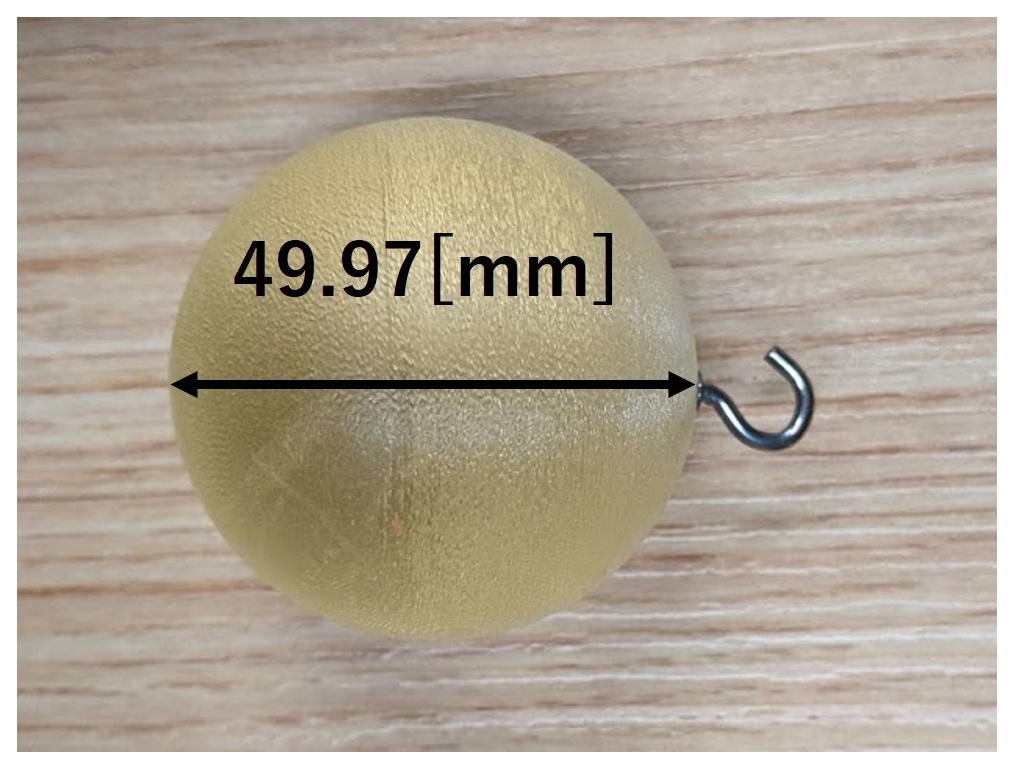
\includegraphics[scale=0.4]{../fig/eps/ball.eps}}
\hspace{7mm}
\\
\subfloat[円筒]{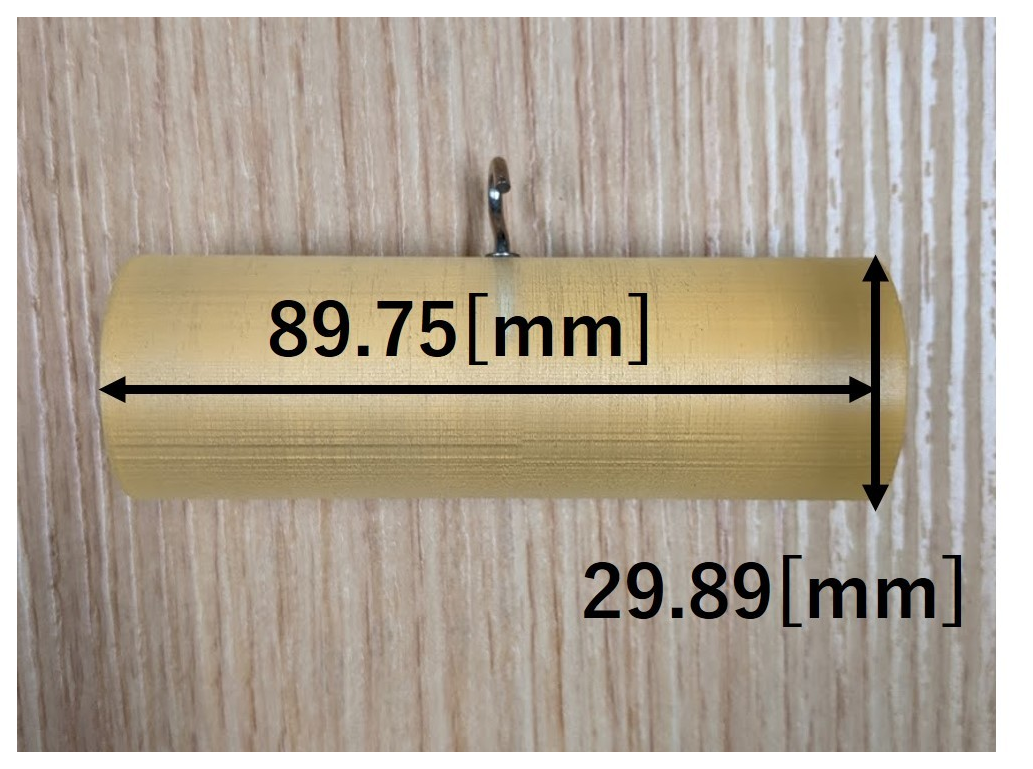
\includegraphics[scale=0.4]{../fig/eps/pole.eps}}
\hspace{7mm}
\subfloat[ボトル]{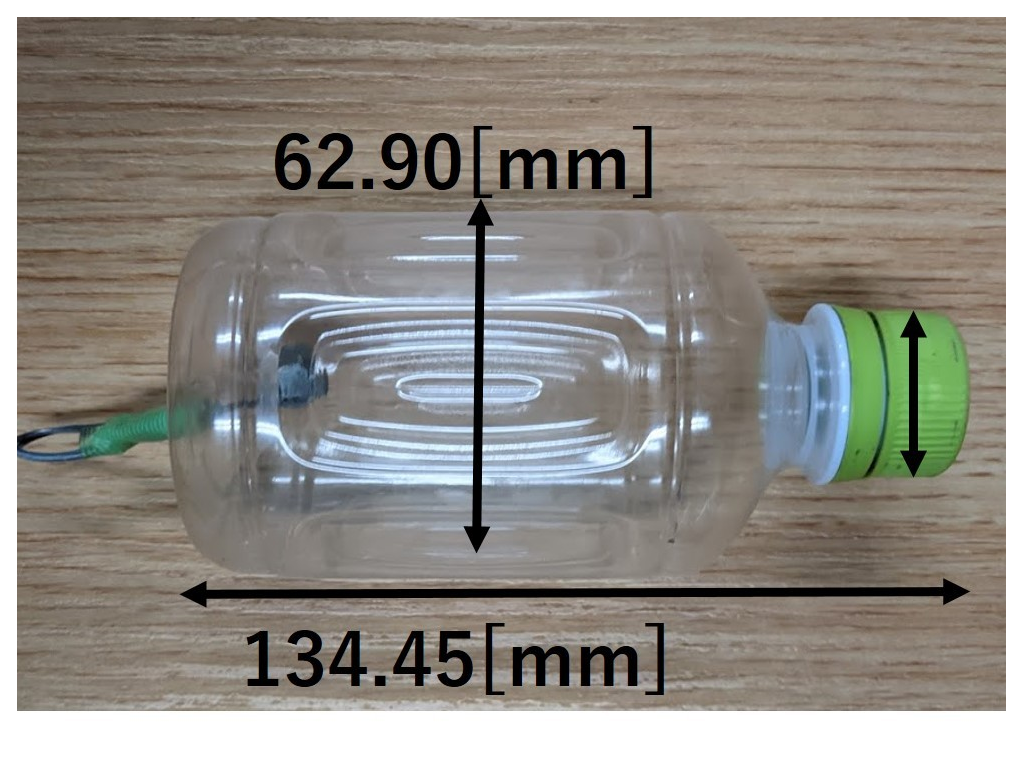
\includegraphics[scale=0.4]{../fig/eps/bottle.eps}}
\hspace{7mm}
\caption{把持対象物}
\label{fig::obj}
\end{figure}

\begin{figure}[h]
 \begin{center}
  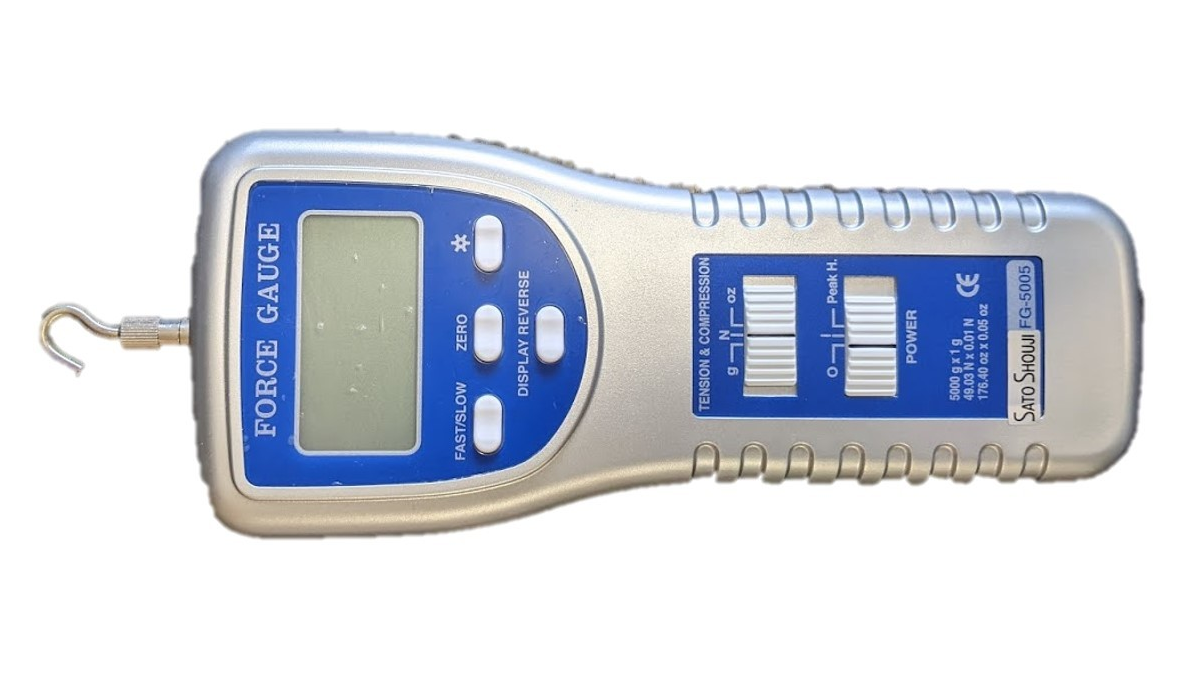
\includegraphics[scale=0.4]{../fig/eps/force_gauge.eps}
 \caption{フォースゲージ}
  \label{fig::force_gauge}
 \end{center}
\end{figure}
\newpage

\subsubsection{センサ使用回路}
イナストマーで力計測をするための専用ソフトウェアである.\refig{ina_kairo}に示す専用回路をPCとUSB接続して用いる.イナストマー購入時に付属される.


\subsubsection{産業用ロボット}
本実験で使用した産業用ロボット(株式会社デンソー製VS087)を\refig{robo}に示す.


\begin{figure}[h]
 \begin{center}
  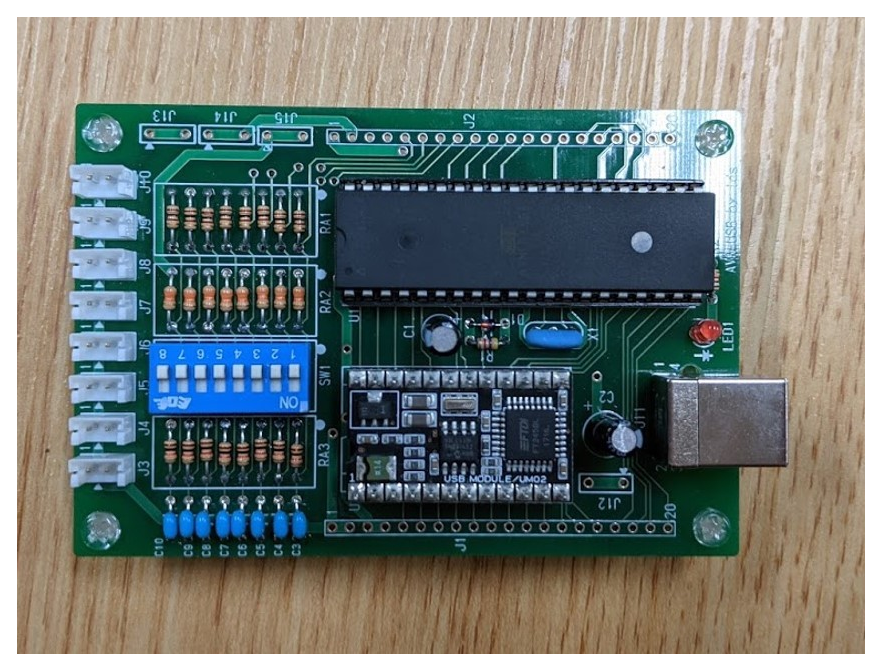
\includegraphics[scale=0.5]{../fig/eps/ina_kairo.eps}
 \caption{専用回路}
  \label{fig::ina_kairo}
 \end{center}
\end{figure}

\begin{figure}[h]
 \begin{center}
  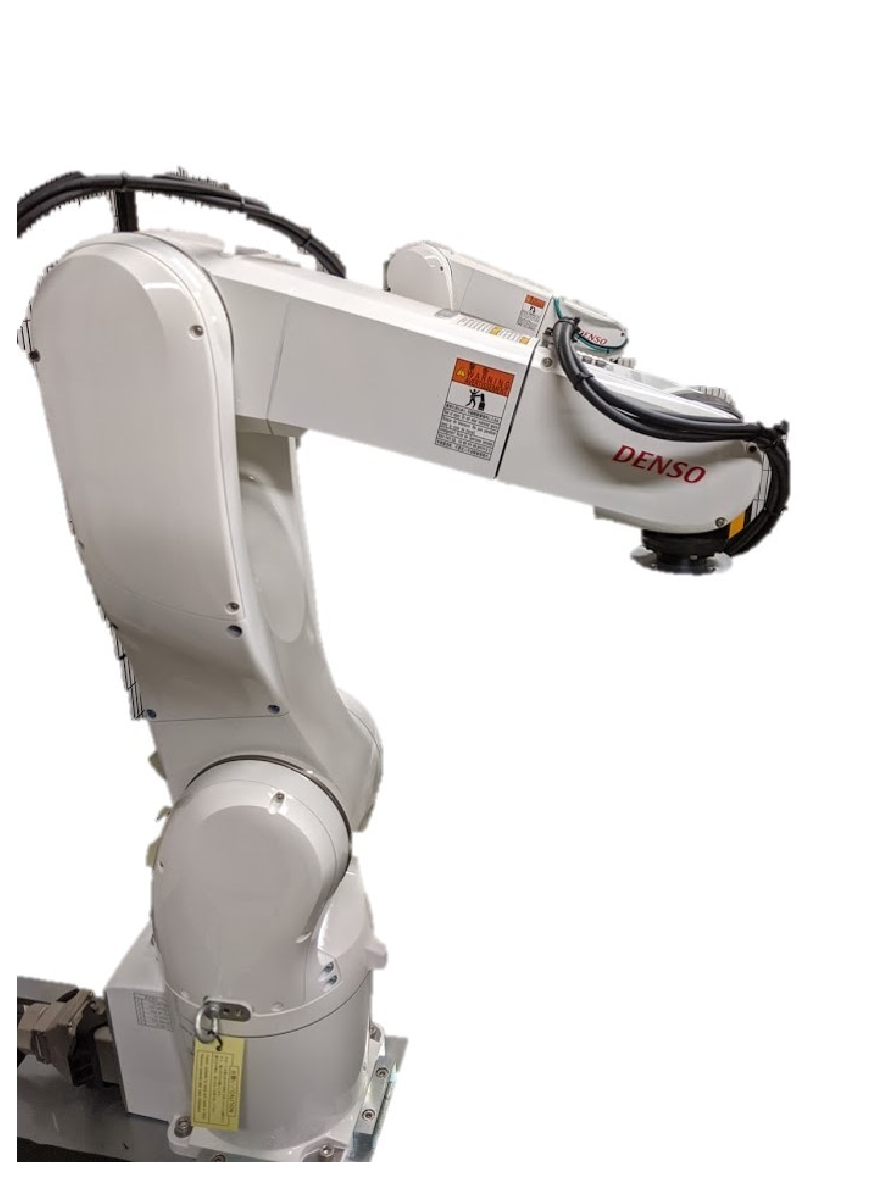
\includegraphics[scale=0.5]{../fig/eps/robo.eps}
 \caption{産業用ロボット}
  \label{fig::robo}
 \end{center}
\end{figure}

\newpage

\subsection{把持実験}
\subsubsection{基礎実験}
力覚センサを組み込んだ柔軟指5秒間把持対象物を把持したときのセンサの応答を検証した.計測誤差結果を\refig{result_sf},\refig{result_sm}に示す.

\subsubsection{荷重実験}
グリッパの把持力を増加させた時の力覚センサの応答を計測した.結果を\refig{result_e2_sf},\refig{result_e2_sm}に示す.

\subsubsection{引張実験}
把持した対象物を鉛直下向きにフォースゲージで引っ張り把持対象物が動いたときの静止摩擦力を計測した.荷重実験と同様にグリッパの把持力を増加させ繰り返した.結果を\refig{result_e3}を示す.


\begin{figure}[htbp]
\centering
\subfloat[球]{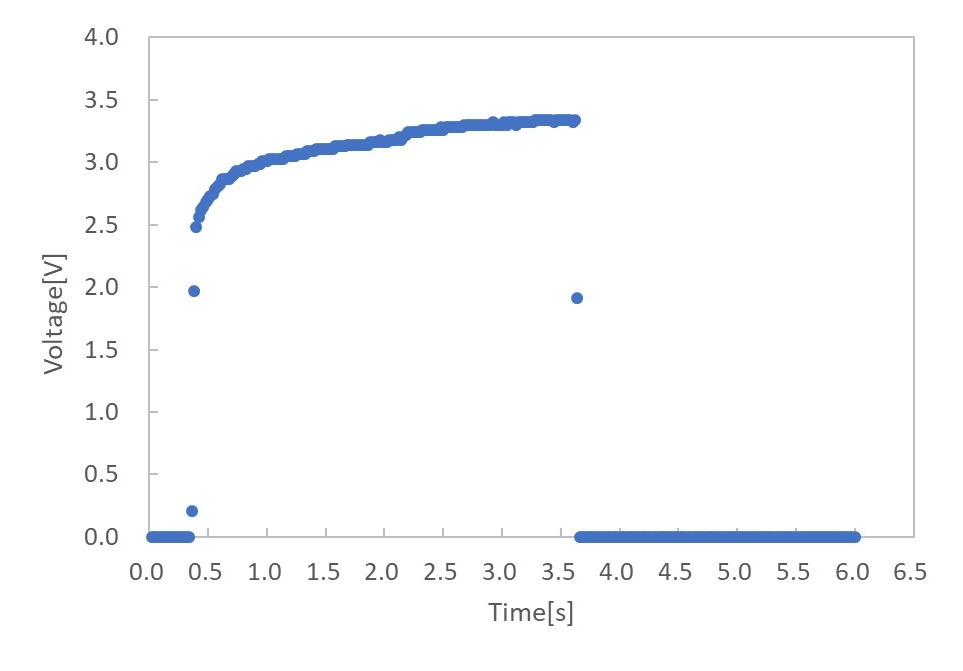
\includegraphics[scale=0.5]{../fig/eps/e0_sf_ball.eps}}
\hspace{5mm}\\
\subfloat[円筒]{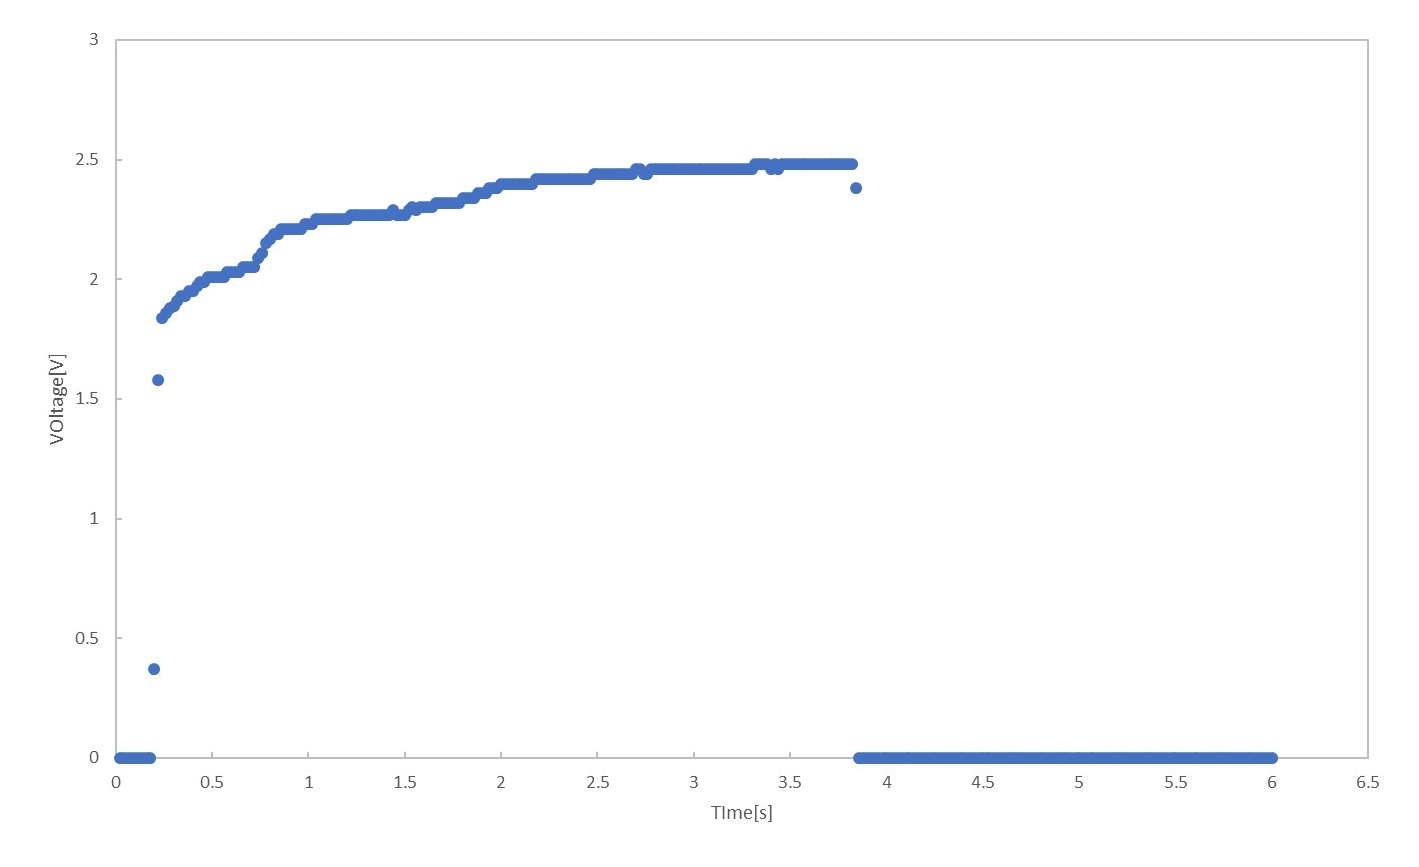
\includegraphics[scale=0.5]{../fig/eps/e0_sf_pole.eps}}
\hspace{5mm}\\
\subfloat[ボトル]{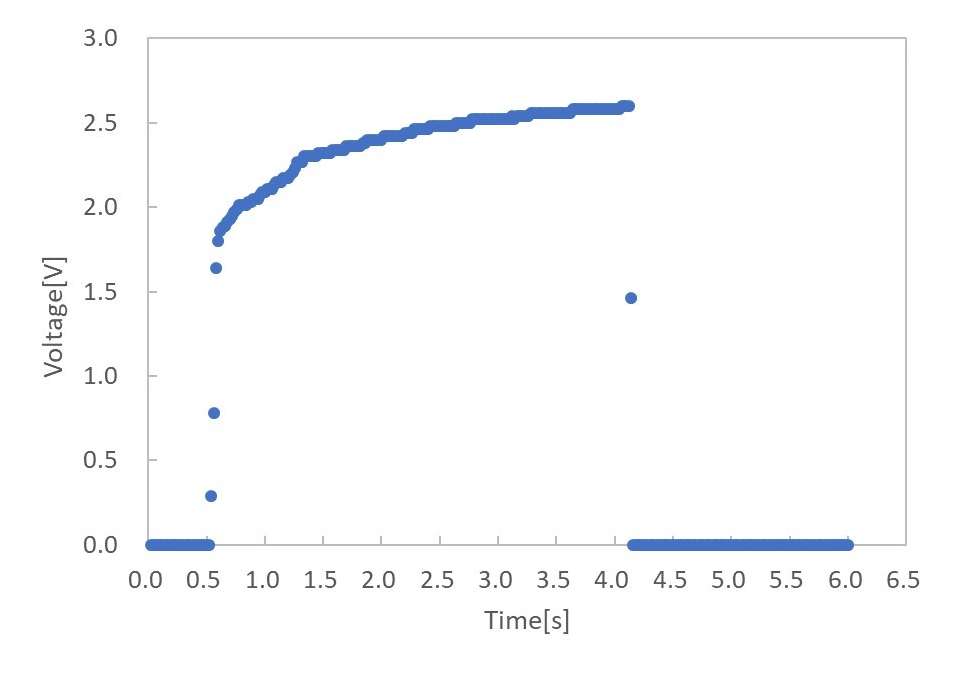
\includegraphics[scale=0.5]{../fig/eps/e0_sf_bottle.eps}}
\hspace{5mm}\\
\caption{把持実験結果(通常指)}
\label{fig::result_sf}
\end{figure}

\clearpage

\begin{figure}[htbp]
\centering
\subfloat[球]{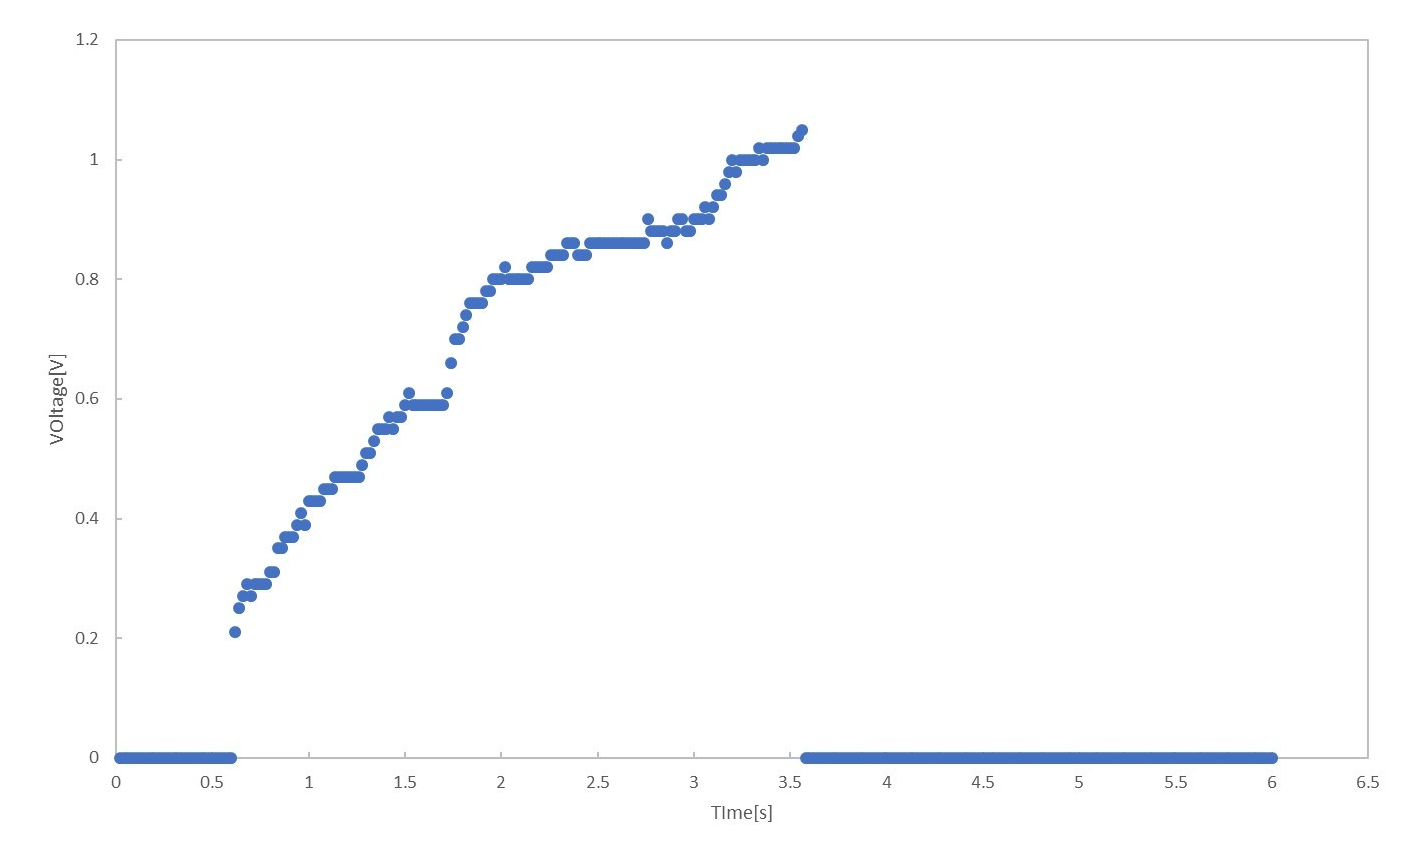
\includegraphics[scale=0.5]{../fig/eps/e0_sm_ball.eps}}
\hspace{5mm}\\
\subfloat[円筒]{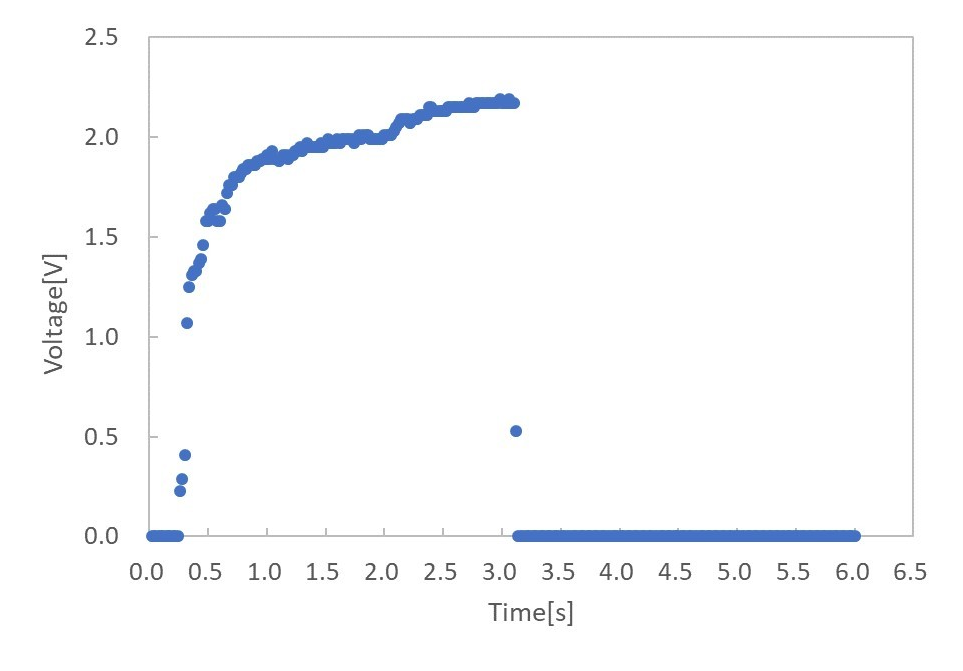
\includegraphics[scale=0.5]{../fig/eps/e0_sm_pole.eps}}
\hspace{5mm}\\
\subfloat[ボトル]{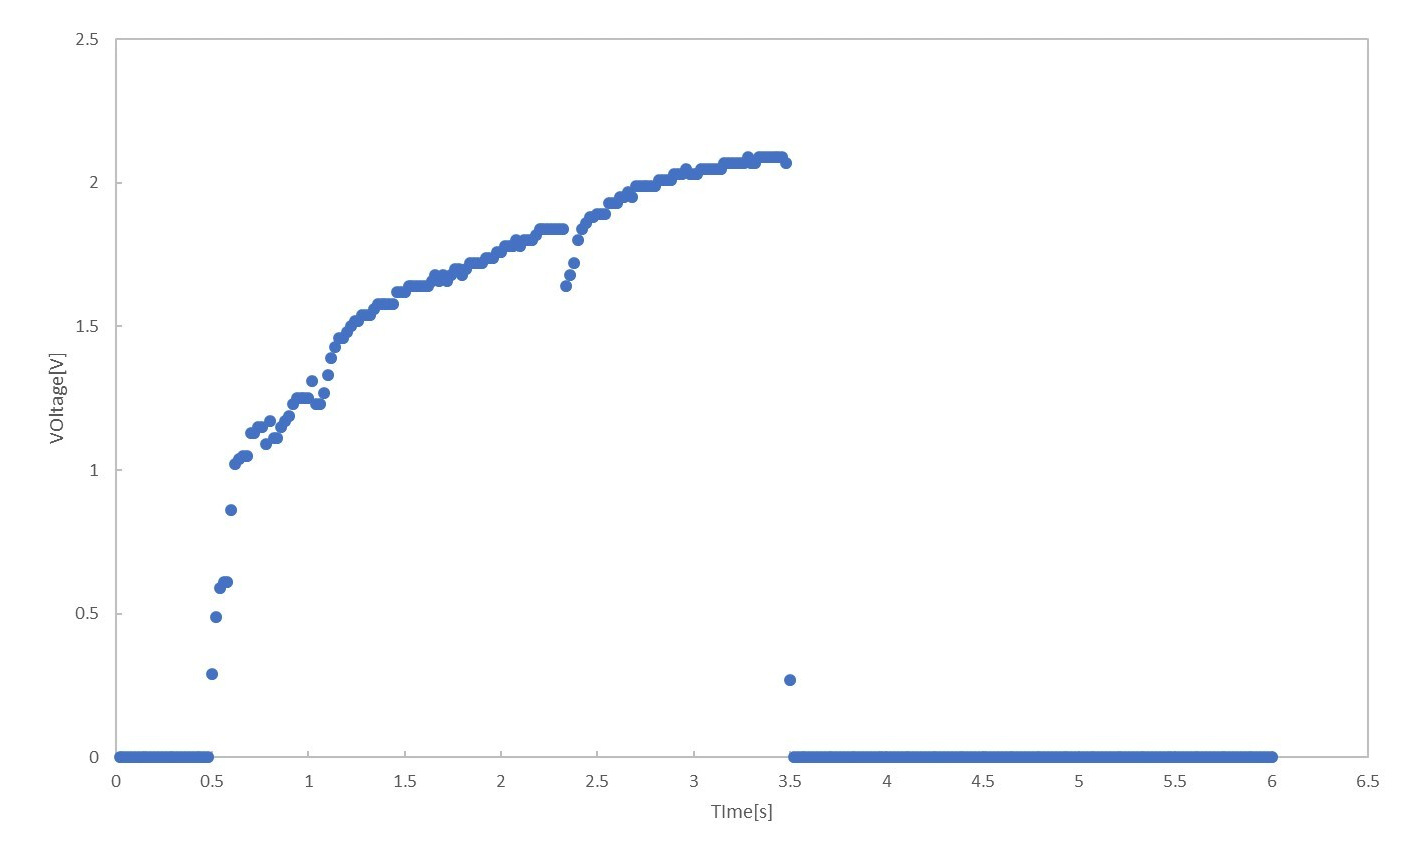
\includegraphics[scale=0.5]{../fig/eps/e0_sm_bottle.eps}}
\hspace{5mm}
\caption{把持実験結果(半球型指)}
\label{fig::result_sm}
\end{figure}

\clearpage



\begin{figure}[htbp]
\centering
\subfloat[球]{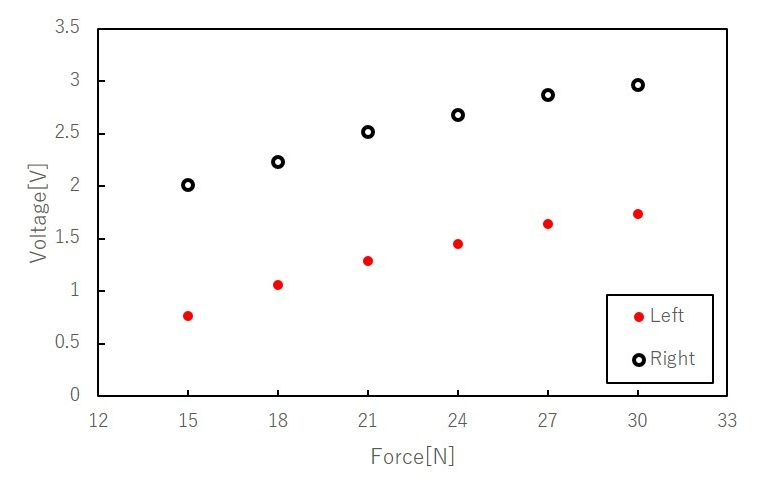
\includegraphics[scale=0.85]{../fig/eps/e2_sf_ball.eps}}
\hspace{5mm}\\
\subfloat[円筒]{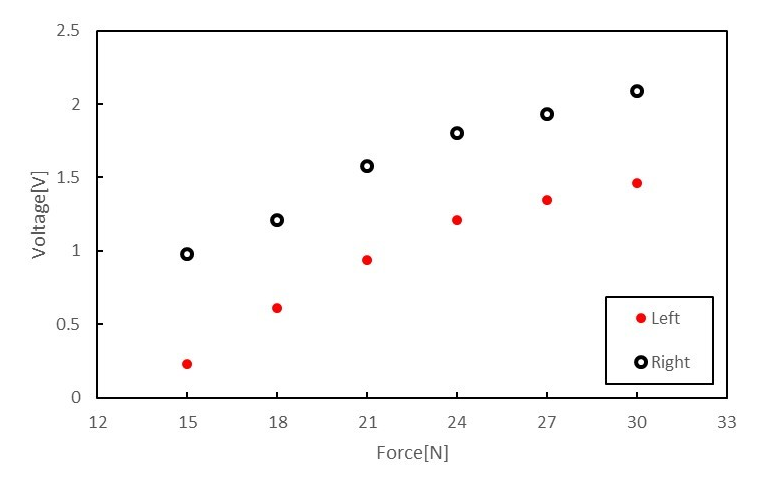
\includegraphics[scale=0.85]{../fig/eps/e2_sf_pole.eps}}
\hspace{5mm}\\
\subfloat[ボトル]{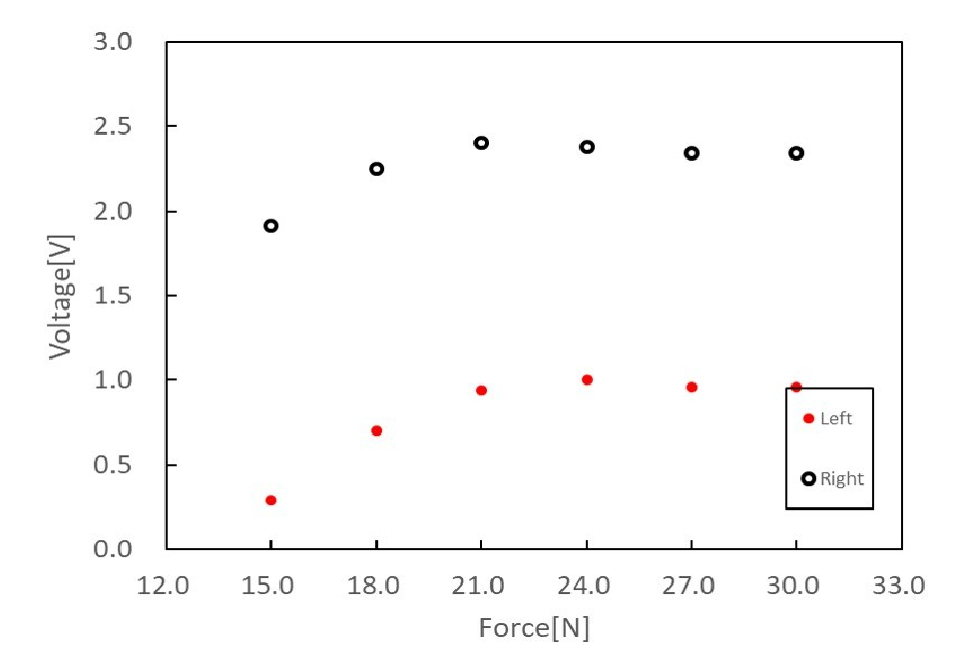
\includegraphics[scale=0.85]{../fig/eps/e2_sf_bottle.eps}}
\hspace{5mm}\\
\caption{荷重実験結果(通常指)}
\label{fig::result_e2_sf}
\end{figure}

\clearpage

\begin{figure}[htbp]
\centering
\subfloat[球]{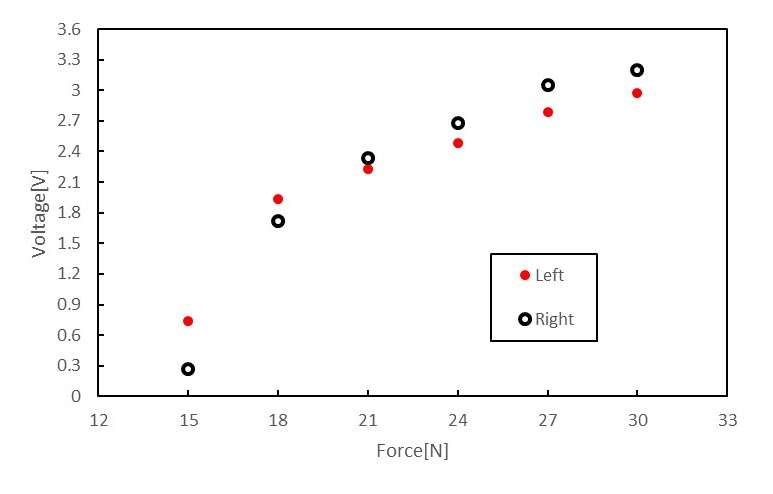
\includegraphics[scale=0.85]{../fig/eps/e2_sm_ball.eps}}
\hspace{5mm}\\
\subfloat[円筒]{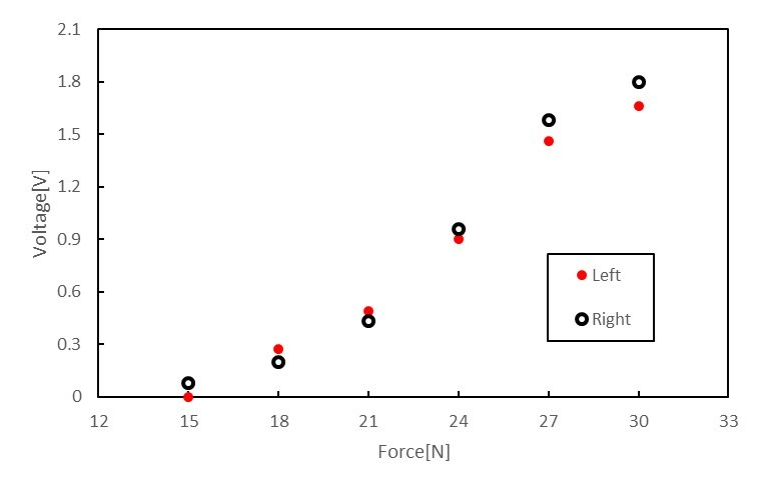
\includegraphics[scale=0.85]{../fig/eps/e2_sm_pole.eps}}
\hspace{5mm}\\
\subfloat[ボトル]{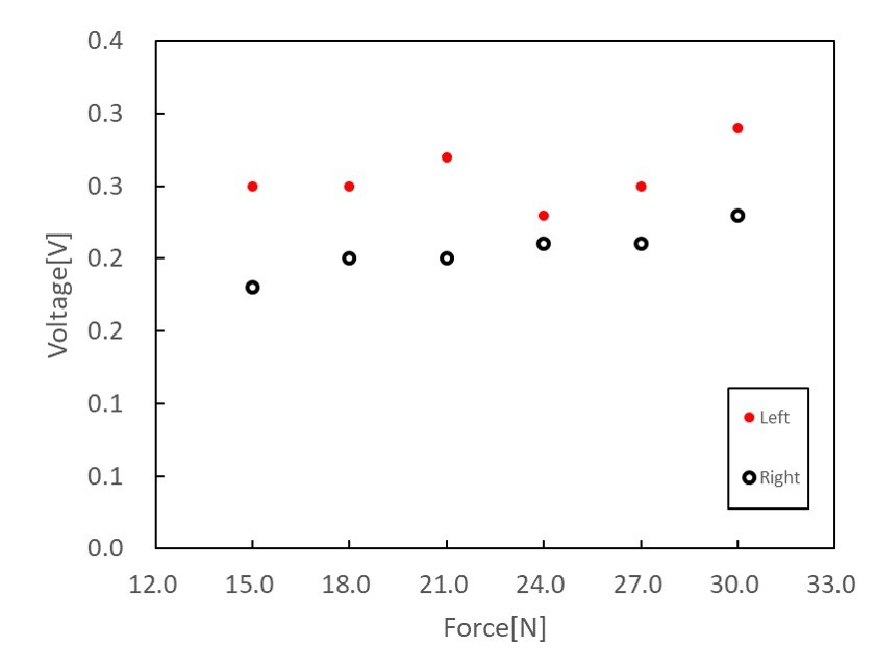
\includegraphics[scale=0.85]{../fig/eps/e2_sm_bottle.eps}}
\hspace{5mm}\\
\caption{荷重実験結果(半球型指)}
\label{fig::result_e2_sm}
\end{figure}

\clearpage

\begin{figure}[htbp]
\centering
\subfloat[球]{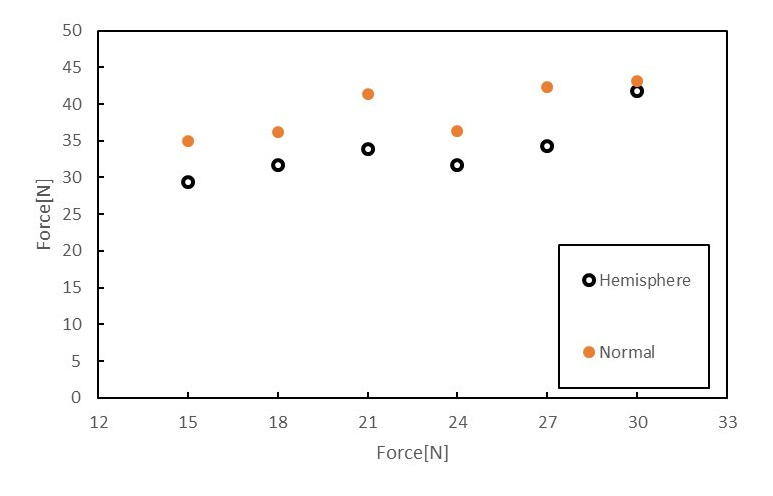
\includegraphics[scale=0.85]{../fig/eps/e3_ball.eps}}
\hspace{5mm}\\
\subfloat[円筒]{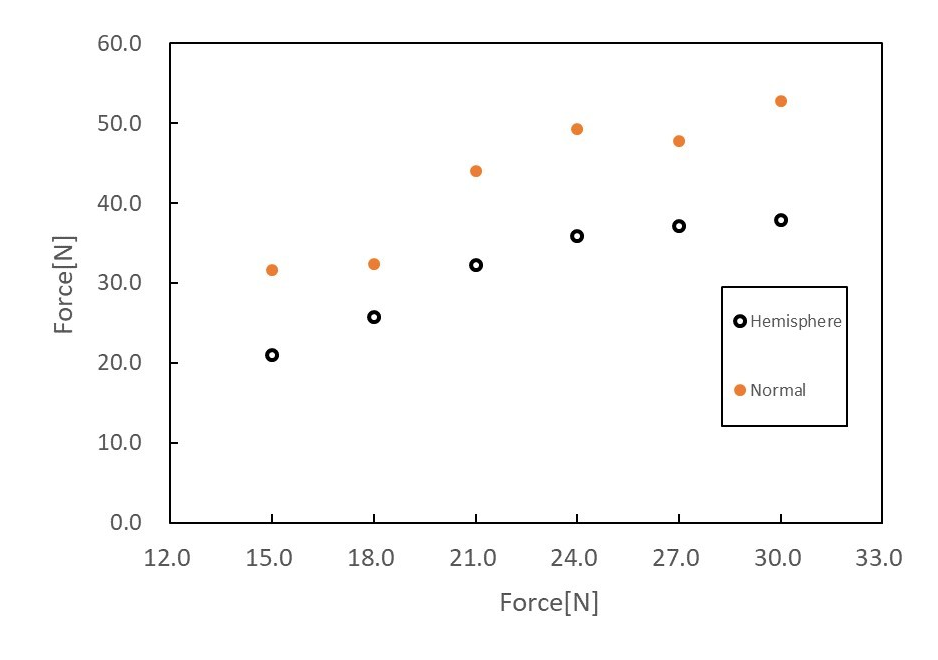
\includegraphics[scale=0.85]{../fig/eps/e3_cylinder.eps}}
\hspace{5mm}\\
\subfloat[ボトル]{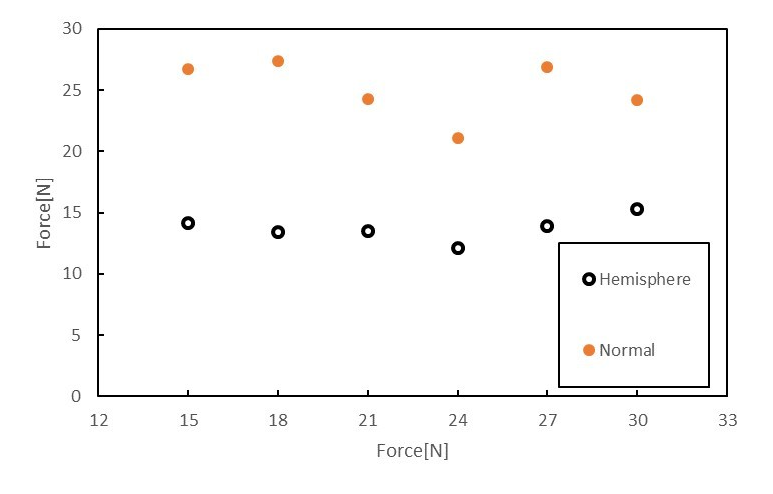
\includegraphics[scale=0.85]{../fig/eps/e3_bottle.eps}}
\hspace{5mm}\\
\caption{引張実験結果}
\label{fig::result_e3}
\end{figure}

\clearpage


